%% MODELO DE LATEX PARA TRABALHOS ACADÊMICOS

\documentclass[
	% -- opções da classe memoir --
	12pt,				% tamanho da fonte
	% openright,			% capítulos começam em pág ímpar (insere página vazia caso preciso)
    oneside,			% para impressão somente frente. Oposto a twoside (frente e verso)
	a4paper,			% tamanho do papel. 
	% -- opções da classe abntex2 --
	%chapter=TITLE,		% títulos de capítulos convertidos em letras maiúsculas
	%section=TITLE,		% títulos de seções convertidos em letras maiúsculas
	%subsection=TITLE,	% títulos de subseções convertidos em letras maiúsculas
	%subsubsection=TITLE,% títulos de subsubseções convertidos em letras maiúsculas
	% -- opções do pacote babel --
	english,			% idioma adicional para hifenização
	french,				% idioma adicional para hifenização
	spanish,			% idioma adicional para hifenização
	brazil,				% o último idioma é o principal do documento
	]{abntex2}


% ---
% PACOTES
% ---

% ---
% Pacotes fundamentais 
% ---
\usepackage{graphicx,url}
\usepackage{graphicx,url}

\usepackage[utf8]{inputenc}
\usepackage[brazil]{babel}
\usepackage{float}
\usepackage{footnote}
\usepackage{graphicx}
\usepackage[most]{tcolorbox}
\usepackage{graphicx,url}
\usepackage[export]{adjustbox}
\usepackage[utf8]{inputenc}
\usepackage[brazil]{babel}
\usepackage{float}
\usepackage{footnote}
\usepackage{graphicx}
\usepackage{array}
\usepackage[most]{tcolorbox}
\usepackage{graphicx,url}
\usepackage{booktabs,chemformula}
\usepackage[export]{adjustbox}
\usepackage{float}
\usepackage{cmap}				% Mapear caracteres especiais no PDF
\usepackage{lmodern}			% Usa a fonte Latin Modern
\usepackage[T1]{fontenc}		% Selecao de codigos de fonte.
\usepackage[utf8]{inputenc}		% Codificacao do documento (conversão automática dos acentos)
\usepackage{indentfirst}		% Indenta o primeiro parágrafo de cada seção.
\usepackage{color}				% Controle das cores
\usepackage{graphicx}			% Inclusão de gráficos
\usepackage{epigraph}
\usepackage{booktabs}
\usepackage{multicol}
\usepackage{multirow}
\usepackage{lipsum}				% para geração de dummy text
\usepackage[brazilian,hyperpageref]{backref}	 % Paginas com as citações na bibl
\usepackage[alf]{abntex2cite}	% Citações padrão ABNT
\usepackage{natbib}

\graphicspath{{./figs/}}

% --- 
% CONFIGURAÇÕES DE PACOTES
% --- 

% ---
% Configurações do pacote backref
% Usado sem a opção hyperpageref de backref
\renewcommand{\backrefpagesname}{Citado na(s) página(s):~}
% Texto padrão antes do número das páginas
\renewcommand{\backref}{}
% Define os textos da citação
\renewcommand*{\backrefalt}[4]{
	\ifcase #1 %
		Nenhuma citação no texto.%
	\or
		Citado na página #2.%
	\else
		Citado #1 vezes nas páginas #2.%
	\fi}%
% ---

% ---
% Informações de dados para CAPA e FOLHA DE ROSTO
% ---
\titulo{Uma interface web para uma aplicação de apresentação de resultados de coleta de questionários customizados georreferenciados}
\autor{Erika Laiane Figueredo do Nascimento e Silva}
\local{Picos - PI}
\data{5 de junho de 2017}
\instituicao{%
  Universidade Federal do Piauí
  \par
  Campus Senador Helvídio Nunes de Barros 
  \par
  Bacharelado em Sistemas de Informação}
\tipotrabalho{Relatório técnico}
% O preambulo deve conter o tipo do trabalho, o objetivo, 
% o nome da instituição e a área de concentração 
\preambulo{Modelo de Trabalho de Conclusão de Curso em Bacharelado em Sistemas de Informação na Universidade Federal do Piauí.
	Este modelo está em conformidade com as normas ABNT.}
% ---

% ---
% Configurações de aparência do PDF final

% alterando o aspecto da cor azul
\definecolor{blue}{RGB}{41,5,195}

% informações do PDF
\makeatletter
\hypersetup{
     	%pagebackref=true,
		pdftitle={\@title}, 
		pdfauthor={\@author},
    	pdfsubject={\imprimirpreambulo},
	    pdfcreator={LaTeX with abnTeX2},
		pdfkeywords={abnt}{latex}{abntex}{abntex2}{relatório técnico}, 
		colorlinks=true,       		% false: boxed links; true: colored links
    	linkcolor=blue,          	% color of internal links
    	citecolor=blue,        		% color of links to bibliography
    	filecolor=magenta,      		% color of file links
		urlcolor=blue,
		bookmarksdepth=4
}
\makeatother
% --- 


% ---
% compila o indice
% ---
\makeindex
% ---







% ----
% Início do documento
% ----
\begin{document}

% Retira espaço extra obsoleto entre as frases.
\frenchspacing 

% ----------------------------------------------------------
% ELEMENTOS PRÉ-TEXTUAIS
% ----------------------------------------------------------
% \pretextual

% ---
% Capa
% ---
\imprimircapa
% ---

% ---
% Folha de rosto
% (o * indica que haverá a ficha bibliográfica)
% ---
\imprimirfolhaderosto*
% ---






% ---
% Agradecimentos
% ---
\begin{agradecimentos}
Insira seus agradecimentos aqui.
\end{agradecimentos}
% ---

% ---
% Epigrafe
% ---
\vspace*{\fill}
{ \raggedleft
	\textit{A tarefa não é tanto ver aquilo que ninguém viu, mas pensar o que ninguém ainda pensou sobre aquilo que todo mundo vê. \\
		Arthur Schopenhauer}
	~
}
\pagebreak


% ---
% RESUMO
% ---

% resumo na língua vernácula (obrigatório)
\begin{resumo} %% AQUI COMEÇA A PÁGINA DE RESUMO
 

 
 % No Resumo precisa ser um pouco mais abrangente mantendo a objetividade das linhas já escritas.

 \vspace{\onelineskip}
    
 \noindent
 \textbf{Palavras-chaves}: latex. abntex. editoração de texto.
\end{resumo} %AQUI TERMINA A PÁGINA DE RESUMO


\begin{resumo}[Abstract]

  
    
\end{resumo}


% ---
% inserir lista de ilustrações
% ---

\listoffigures* %% o * indica que não será incluso no sumário
\cleardoublepage %% Pula página
% ---

% ---
% inserir lista de tabelas
% ---

\listoftables*
\cleardoublepage
% ---

% ---
% inserir lista de abreviaturas e siglas
% ---
\begin{siglas}
  \item[Fig.] Area of the $i^{th}$ component
  \item[456] Isto é um número
  \item[123] Isto é outro número
  \item[lauro cesar] este é o meu nome
\end{siglas}
% ---

% ---
% inserir lista de símbolos
% ---
\begin{simbolos}
  \item[$ \Gamma $] Letra grega Gama
  \item[$ \Lambda $] Lambda
  \item[$ \zeta $] Letra grega minúscula zeta
  \item[$ \in $] Pertence
\end{simbolos}
% ---

% ---
% inserir o sumario
% ---

\tableofcontents*

% ---

% ----------------------------------------------------------
% ELEMENTOS TEXTUAIS  (necessário para incluir número nas páginas)
% ----------------------------------------------------------
\textual


% ----------------------------------------------------------
% Introdução
% ----------------------------------------------------------
\chapter{Introdução} %% NOVO CAPÍTULO (REPARE QUE ELE AUTOMATICAMENTE JÁ COLOCA O NÚMERO DO CAPÍTULO E JÁ ADICIONA NO SUMÁRIO)

Podemos destacar um aumento na demanda por informação geoespacial em diversas atividades rotineiras; não é difícil deparar-se com situações que necessitam do uso da tecnologia, seja para comunicação, entretenimento, informação e também por localização. Isso se deu devido a crescente popularização dos dispositivos móveis como smartphones e tablets, munidos de aplicações que fazem uso da localização de seus usuários. Podemos citar, dentre eles, o WhatsApp, para compartilhar a localização do usuário, o próprio Facebook, que utiliza o serviço de localização, o Google Maps, dentre outros. Sendo assim, para administrar as informações, são utilizadas técnicas de tratamento computacional de dados geográficos, com o objetivo de levar a resoluções de possíveis problemas e tomada de decisão.

A pesquisa de campo é o principal método de coleta de dados. Baseia-se no estudo de indivíduos, grupos, com o objetivo de melhor entender as diferentes características de uma determinada comunidade e realizar um levantamento de informações sobre um determinado problema. Os questionários são as técnicas de investigação mais utilizadas nas pesquisas de campo e são utilizados como recursos instrumentais em pesquisas sobre assuntos específicos.

“O termo Sistemas de Informação Geográfica (SIG) é aplicado para sistemas que realizam o tratamento computacional de dados geográficos” (CÂMARA, 2005). Dados geográficos ou georreferenciados são dados em que a dimensão do espaço está relacionada à sua localização na superfície da terra. Um SIG é composto por um conjunto de programas computacionais o qual integra dados, equipamentos e pessoas com objetivo de coletar, armazenar, recuperar, manipular, visualizar e analisar dados espacialmente referenciados a um sistema de coordenadas conhecido. 
Geoprocessamento consiste em armazenar a geometria e os atributos de dados georreferenciados descrevendo características, limitações de mapas ou imagens, tornando assim, qualquer forma de informação geográfica conhecida em um banco de dados.

A proposta deste trabalho está incluída em um projeto maior. O projeto está relacionado a uma arquitetura para coleta de questionários customizados divididos em quatro módulos: um banco de dados geográficos acoplado para armazenamento dos dados espaciais coletados, uma ferramenta SIG para suporte e manipulação das informações geográficas, uma aplicação Android para coleta dos dados dos questionários e uma \textit{Interface Web} para visualização e manipulação. Tanto o banco de dados quanto a ferramenta SIG já foram implementados e testados.

O trabalho visou à criação de uma interface web que visualize dados coletados por uma ferramenta de coleta móvel. Essa ferramenta será apropriada para coletar os dados espaciais feito pelos pesquisadores utilizando dispositivos móveis para Android, constituindo um outro módulo do projeto ainda em desenvolvimento. Os dados referentes ao questionário, além dos dados espaciais serão armazenados. Essa interface ficará responsável por prover meios para exibir a distribuição espacial destes dados coletados.


\section{Objetivo}
O objetivo desse trabalho consiste no desenvolvimento de uma \textit{interface} de um sistema \textit{web} para prover meios de visualizações de consultas de informações geográficas e a distribuição espacial dos dados coletados por uma aplicação de coleta de questionários customizados.

\section{Organização do trabalho}
O presente trabalho está organizado em 5 (cinco) capítulos. Após a introdução, que apresentou o problema que se pretende resolver e o objetivo, os próximos capítulos estão organizados da seguinte forma: 
\begin{itemize}
    \item Capítulo 2 – Referencial Teórico: São apresentados os conceitos relacionados ao Sistemas de Informação geográficos, atividade de pesquisa de campo, e os trabalhos da literatura, fornecendo a sustentação teórica da proposição;
    \item Capítulo 3 – Trabalhos Relacionados: São apresentados alguns trabalhos que demonstram semelhanças com a proposta;
    \item Capítulo 4 – Desenvolvimento da Aplicação: Apresentação dos requisitos necessários para a realização da \textit{Interface web};
    \item Capítulo 5 – Conclusão: Apresenta a conclusão do trabalho e sugestão de trabalhos futuros.
\end{itemize}
	
% ---
% Capitulo de revisão de literatura
% ---
\chapter{Referencial Teórico}
A fim de obter uma concepção clara do presente trabalho, serão apresentados os conceitos em relação aos principais itens que abordam a atividade de Geoprocessamento, Sistema de Informação Geográfica, Sistemas de Informação geográficas na \textit{web}, atividade de pesquisa de campo onde serão empregados no desenvolvimento de uma aplicação de coleta de questionários customizados.

% --- Seção dentro do capítulo
\section{Geoprocessamento}
O Geoprocessamento é um conjunto de tecnologias que engloba a coleta, o tratamento, a manipulação, e apresentação de informações espaciais voltado para um objetivo em específico (CÂMARA). O sistema de Geoprocessamento engloba todos os sistemas computacionais capazes de processar dados georreferenciados, como exemplo, os sistemas de cartografia automatizada e os sistemas de CAD (Projeto Auxiliado por Computador), porém possui como principal ferramenta o Sistemas de Informação Geográfica que realiza as atividades que envolve o geoprocessamento de dados auxiliando muitas vezes nas tomada de decisões. 

(GOMES) Justifica que o Geoprocessamento representa a área do conhecimento que utiliza técnicas matemáticas e computacionais para tratar a informação geográfica e SIG como ferramenta computacional para o processamento, integrando dados de diversas fontes de dados georreferenciados resultado em conteúdo para possíveis tomadas de decisões estratégicas.

O Geoprocessamento surgiu devido ao elevado crescimento das tecnologias de \textit{software} e \textit{hardware} aplicadas ao gerenciamento de informações e processamento de dados e imagens geográficas. O objetivo era automatizar parte do processamento de dados com características espaciais, diminuindo custos de produção e manutenção de mapas, principalmente quando comparados ao da produção manual, uma vez que esta emprega mídias físicas como o papel, que podem se tornar caras principalmente considerando os aspectos de armazenamento e atualização parte do processamento de dados (RECKZIEGEL, 2009).

Os dados manipulados pelas aplicações de Geoprocessamento são chamadas de dados georreferenciados. Georreferenciamento é a técnica de manipulação dos dados aplicados pelo geoprocessamento (REFERÊNCIA), responsável por tornar as coordenadas de dados de informação geográfica visíveis, estando relacionados a localização geográfica na superfície da terra. Podendo ser representados por uma imagem ou mapa entre outras formas onde um sistema de geoprocessamento desempenha a função de armazená-los.

O processo de obtenção de dados georreferenciados é realizado pelo \textbf{Sensoriamento Remoto}. É um termo utilizado na área das ciências aplicadas que se refere à obtenção de imagens à distância, sobre a superfície terrestre. De acordo com (referência) é definido como a ciência e a arte de se obter informações sobre objetos, áreas ou fenômenos, através da análise dos dados adquiridos por um dispositivo que não esteja em contato com o objeto, área ou fenômeno sob investigação. O GPS (Global Positioning System – Sistema de Posicionamento Global) é um sistema de posicionamento por satélite que fornece a um aparelho receptor móvel a sua posição geográfica.

\section{Sistema de Informação Geográfica}
Sistemas de Informação Geográfica são ferramentas computacionais para geoprocessamento, construídos especialmente para armazenar, analisar e manipular dados geográficos, ou seja, dados que representam objetos e fenômenos cujo tratamento prescinde da localização geográfica (CÂMARA, 2005). 

De acordo com (furquim) O SIG pode ser considerado um sistema que realiza o tratamento computacional de dados geográficos e recuperam informações, não apenas com base em suas características alfanuméricas, mas também através de sua localização espacial; oferece aos administradores e técnicos uma visão ampla do ambiente de atuação, na qual as informações disponíveis estão ao seu alcance, inter-relacionadas com base num aspecto comum que é a sua localização geográfica. 

Um SIG pode possuir duas categorias básicas de dados: \textbf{dados convencionais} - atributos alfanuméricos usados para armazenar os dados descritivos e temporais; e \textbf{dados espaciais} - atributos que descrevem a geometria, a localização geográfica e os relacionamentos espaciais. 

Os SIGs se diferenciam dos demais sistemas que manipulam dados georreferenciados, como CAD, por dois motivos principais: Primeiro, por sua capacidade de representar os relacionamentos espaciais (ou topológicos) entre fenômenos geográficos. Segundo, por permitir a realização de complexas operações de análise espacial com os dados geográficos (JUGURTA). Permitindo aos usuários a realização dessas operações.

Ainda de acordo com (JUgurta 1996) os SIGs se destacam por permitir manipular dados gráficos e não-gráficos de forma integrada. Dados gráficos(\textit{pixels}, pontos, linhas) são utilizados para representar elementos gráficos geograficamente. Pode-se permitir, por exemplo, acesso a registros de imóveis a partir de sua localização geográfica. Como também, podem fazer conexões entre diferentes entidades, baseados no conceito de proximidade geográfica.
 
(Burrough) também afirma que os SIGs correspondem às ferramentas computacionais de Geoprocessamento, que permitem a realização de análises complexas, ao integrar dados de diversas fontes e ao criar bancos de dados georreferenciados. Ainda acrescenta que estes sistemas não apresentam apenas a função de manipulação de dados geográficos, mas, dentro de um SIG, os dados estruturados representam um modelo do mundo real.

(PEDROSA) ainda relata que os SIGs constituem o tipo de estrutura mais importante em termos de viabilização do geoprocessamento. Logo, é uma ferramenta de grande utilidade e crescente disponibilidade, que provê facilidade de acesso e análise de dados mediante sistemas computacionais. 

Um SIG pode ser visto como uma representação simplificada digital das características da terra para uma determinada região. Os dados georreferenciados podem ser organizados dentro do SIG utilizando diferentes critérios, por exemplo, como camadas temáticas ou objetos espaciais (CRUZ; CAMPOS, 2005).


\begin{figure} [H]
%% hbt SIGNIFICA QUE ELE PRIMEIRO VAI TENTAR COLOCAR A IMAGEM NESTE LUGAR (h de "here"). SENÃO DER, ELE TENTA COLOCAR MAIS PRA BAIXO (b de "bottom"). SENÃO ELE COLOCA MAIS PARA CIMA (t de "top").
\label{figura1} 
%% LABEL SERVE PARA VOCÊ REFERENCIAR A FIGURA NO MEIO DO TEXTO (VEJA LINHA 330: \ref{figura1}). ASSIM VOCÊ NÃO PERDE A REFERÊNCIA QUANDO MUDA A FIGURA DE LUGAR
\caption{Representação das camadas temáticas.}
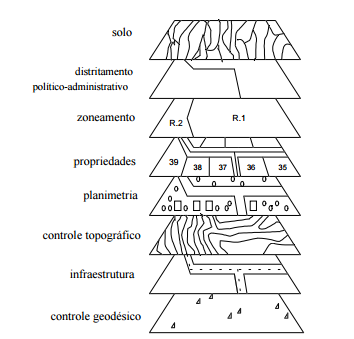
\includegraphics[width=0.95\textwidth]{camadatematica.png} %% PARA COLOCAR O ARQUIVO DA IMAGEM NO SHARELATEX, CLIQUE NO ÍCONE QUE PARECE UMA FLECHINHA PARA CIMA (ATUALIZAR), CLIQUE EM UPLOAD E PROCURE A IMAGEM EM SEU COMPUTADOR.
\end{figure}

Em um SIG, os dados geográficos são estruturados em planos de informação, também denominados de camadas. As camadas quando estão sendo referenciadas geograficamente a algum sistema de coordenadas, sendo eles, topográficas, geográficas, geodésicas ou cartesianas podem ser sobrepostas e representam o mundo real (FRANCISCO et al.,  ). Para que ocorra a correta sobreposição, é necessário encontrar o ponto em comum entre a projeção cartográfica, sistemas de coordenadas e sistema geodésico (DATUM). O DATUM consiste em um sistema de referência e coordenadas associado a características terrestres.



\section{Arquitetura de um SIG}
Devido à grande procura de aplicações SIG em diversas áreas, incluindo aplicações no transporte, na agricultura, na floresta, cartografia entre outros, os SIGs podem ser utilizados de três maneiras distintas. São elas (CÂMARA, 2005).

\begin{itemize}
    \item Como ferramenta para produção de mapas;
    \item Como suporte para análise espacial de fenômenos;
    \item Também como um banco de dados geográficos, com funções de armazenamento e recuperação de informação espacial.
\end{itemize}

A partir das definições, podemos resumir as principais características de um SIG enumeradas por Câmara (2005):

\begin{itemize}
	\item Integrar, numa única base de dados, as informações espaciais provenientes de dados cartográficos; e dados alfanuméricos provenientes de censo e cadastro urbano e rural, imagens de satélite, redes e modelos numéricos de terreno;
	
	\item Oferecer mecanismos para combinar as várias informações, através de algoritmos (instruções) de manipulação e análise, bem como para consultar, recuperar, visualizar e plotar o conteúdo da base de dados georreferenciados.
\end{itemize}


Em uma visão mais ampla, (CÂMARA, 2005) apresenta um SIG possuindo a seguinte arquitetura: 

\begin{figure} [H] 
%% hbt SIGNIFICA QUE ELE PRIMEIRO VAI TENTAR COLOCAR A IMAGEM NESTE LUGAR (h de "here"). SENÃO DER, ELE TENTA COLOCAR MAIS PRA BAIXO (b de "bottom"). SENÃO ELE COLOCA MAIS PARA CIMA (t de "top").
\label{figura1} 
%% LABEL SERVE PARA VOCÊ REFERENCIAR A FIGURA NO MEIO DO TEXTO (VEJA LINHA 330: \ref{figura1}). ASSIM VOCÊ NÃO PERDE A REFERÊNCIA QUANDO MUDA A FIGURA DE LUGAR
\caption{Arquitetura de um Sistema de Informação Geográfica.}
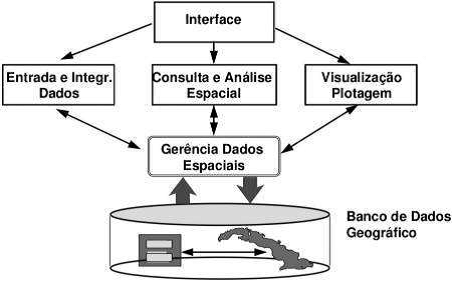
\includegraphics[width=0.95\textwidth]{arquitetura.png} %% PARA COLOCAR O ARQUIVO DA IMAGEM NO SHARELATEX, CLIQUE NO ÍCONE QUE PARECE UMA FLECHINHA PARA CIMA (ATUALIZAR), CLIQUE EM UPLOAD E PROCURE A IMAGEM EM SEU COMPUTADOR.
\end{figure}

\begin{itemize}
    \item Interface – a interface com o usuário contempla as diretrizes de controle e operacionalização do sistema, sendo este o nível que está mais próximo do usuário final;
    \item Entrada e integração de dados - desempenham funções de conversões dos dados geográficos para um formato adequado ao armazenamento;
    \item Consulta e Análise espacial – mecanismos que permitem a realização de cálculos para obtenção de estatísticas espaciais, responsáveis por mapear essa informação no formato de saída;
    \item Visualização e plotagem -  responsável pelo processamento dos dados de entrada e saída, possibilitando a edição, análise e visualização de dados;
    \item Gerenciamento de dados espaciais -  corresponde ao armazenamento recuperação e gerenciamento de dados espaciais, sendo o nível mais interno do sistema.
\end{itemize}

Em uma visão de (baptista) ele separa a arquitetura de um sig em camadas:

\begin{itemize}
    \item Armazenamento: engloba os subsi que oferecem serviços de armazenamento de dados não espaciais, de dados em formato \textit{raster}, de dados em vetor;
    \item Manipulação: oferece funções para definição e manipulação destes objetos;
    \item Visualização: oferece funções básicas para visualização de objetos tradicionais e georreferenciados.
\end{itemize}

Ainda segundo (baptista), existem diferentes estratégias de implementação para a arquitetura em camadas, baseadas em sistemas de gerência de banco de dados com grau crescente de funcionalidade definido com Relacional, Dual e Integrada.

\section{Gerência Dados em um SIG}aOs SIG precisam armazenar grandes quantidades de dados e torná-los disponíveis para operações de consultas e análise (jugurta). Com o aumento na procura por SIG, houve a necessidade de gerenciadores de dados geográficos que armazenam tanto a geometria como também os atributos dos objetos em um Sistemas Gerenciadores de Banco de Dados (SGBD) que são ferramentas fundamentais paro os SIG. Desta forma, o uso de Sistemas de Gerenciamento de Banco de Dados é imprescindível na administração dessas informações.

Existe um grande número de pesquisas na área de banco de dados voltadas a buscar novas formas de gerenciar dados georreferenciados. Atualmente, a estrutura mais utilizada na elaboração dos SIG é a que emprega uma arquitetura dual onde é composto de SGBD relacional, responsável pela gerência dos atributos acoplado a um componente de software responsável pelo gerenciamento dos atributos espaciais (jugurta 1996). 

A seguir uma breve explanação sobre as estratégias para a implementação da arquitetura em camadas segundo (jugurta)

\textbf{Arquitetura Relacional} - Está associado a representação dos temas na forma de relações. Um objeto geográfico é uma tupla ou linha de uma relação. Atributos ou campos são tipos simples capzes de receber valores de texto, inteiros ou geográficos, permitindo uso de \textit{Structured Query Language} (SQL) para consultas aos dados.

FIGURA....

\textbf{Arquitetura Dual} - Um SIG possui um SGBD relacional para armazenar em tabelas, o componente convencional de todos os objetos (dados não espaciais) e arquivos normais para o componente espacial dos objetos. 

De acordo com (Junior e Leal), o modelo Dual tenta solucionar o problema de gerenciamento de dados geográficos integrando os dados convencionais e espaciais, armazenados em bases de dados distintas, através de identificadores comuns as duas bases. (Camara 2001) afirma que essa estratégia tem como principal vantagem a possibilidade de utilização dos SGBDs relacionais do mercado. Entretanto, as principais desvantagens dessa arquitetura é a dificuldade em garantir integridade entre as partes geométricas e descritiva da representação do objeto geográfico; dificuldade na manipulação e no controle dos elementos espaciais.

\begin{figure} [H] 
%% hbt SIGNIFICA QUE ELE PRIMEIRO VAI TENTAR COLOCAR A IMAGEM NESTE LUGAR (h de "here"). SENÃO DER, ELE TENTA COLOCAR MAIS PRA BAIXO (b de "bottom"). SENÃO ELE COLOCA MAIS PARA CIMA (t de "top").
\label{figura1} 
%% LABEL SERVE PARA VOCÊ REFERENCIAR A FIGURA NO MEIO DO TEXTO (VEJA LINHA 330: \ref{figura1}). ASSIM VOCÊ NÃO PERDE A REFERÊNCIA QUANDO MUDA A FIGURA DE LUGAR
\caption{Arquitetura de um Sistema de Informação Geográfica.}
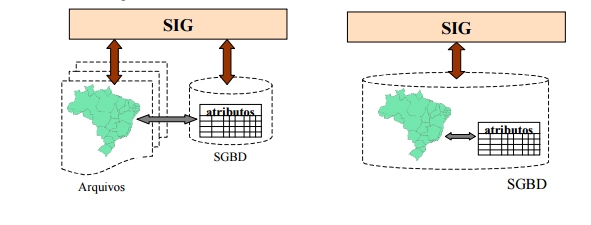
\includegraphics[width=0.95\textwidth]{dual_integrada.png} %% PARA COLOCAR O ARQUIVO DA IMAGEM NO SHARELATEX, CLIQUE NO ÍCONE QUE PARECE UMA FLECHINHA PARA CIMA (ATUALIZAR), CLIQUE EM UPLOAD E PROCURE A IMAGEM EM SEU COMPUTADOR.
\end{figure}

\textbf{Arquitetura Integrada} - De acordo com (Câmara 2005) consiste em armazenar tanto o componente espacial quanto a alfanumérico em um SGBD. (baptista) complementa como sendo o uso de um SGBD extensível (Orientado a Objeto ou Objeto Relacional) que disponha de mecanismos que permitam implementar o tratamento das componentes espaciais através de extensões de acordo com o seu ambiente. Sua principal vantagem é a utilização dos recursos de um SGBD para controle e manipulação de objetos espaciais, como gerência de transações, controle de integridade, concorrência e linguagens próprias de consulta (CÂMARA et al., 2001). Na opinião de (Junior) O modelo de arquitetura Integrada trata-se de uma proposta que se utiliza de tipos de dados definidos pelo usuário e que necessita de implementações que se preoucupem com a melhor forma de armazenamento e recuperação.

Esta última arquitetura ainda pode ser subdividida em outras três: Arquitetura baseada em campos longos; Arquitetura baseada em extensões espaciais; e Arquitetura combinada.

A arquitetura integrada baseada em um SGBD relacional pode ser subdividida em três categorias: Arquitetura baseada em campos longos, Arquitetura baseada em extensões espaciais; e Arquitetura combinada. 



\textbf{Arquitetura baseada em campos longos} - Utiliza campos longos chamados de \textbf{BLOBs}(\textit{Binary Large Object} – Objeto Grande Binário), um conjunto de dados binários armazenados como uma única entidade, para armazenar o elemento espacial dos dados.
 Suas principais desvantagens são:
 
 
\begin{itemize}
    \item Não é capaz de capturar a semântica dos dados espaciais: como o SGBD trata o campo longo como uma cadeia binária, não é possível conhecer a semântica do seu conteúdo;
    \item Métodos de acesso espacial e otimizador de consultas devem ser implementados pelo SIG: como o SGBD trata os dados espaciais como uma cadeia binária, não possui mecanismos satisfatórios para o seu tratamento;
    \item Limitações da linguagem SQL1 para a manipulação dos dados espaciais: a SQL padrão oferece recursos limitados para o tratamento de campos longos.

\end{itemize}

\textbf{Arquitetura baseada em extensões espaciais} -  Estas extensões contêm funcionalidades e procedimentos que permitem armazenar, acessar e analisar dados espaciais de formato vetorial. 
Algumas vantagens:
\begin{itemize}
    \item Permite definir tipos de dados espaciais, equipados com operadores específicos (topológicos e métricos);
    \item Permite definir métodos de acesso específicos para dados espaciais
\end{itemize}
	

Como desvantagens dessa arquitetura podem ser citadas:
\begin{itemize}
    \item Faltas de mecanismos de controle de integridade sobre os dados espaciais;
    \item Falta de padronização das extensões da linguagem SQL.
\end{itemize}

\section{Atividade de Coleta de Dados}
A pesquisa de campo é o principal método de coleta de dados. Baseia-se no estudo de indivíduos, grupos, com o objetivo de melhor entender as diferentes características de uma determinada comunidade e realizar um levantamento de informações sobre um determinado problema. Os cinco métodos mais utilizados na coleta de informação são: questionários, entrevistas, observação direta, registros institucionais e grupos focais (BARBOSA; SILVA, 2010).

Dentre os métodos de coleta mais utilizados:
\begin{itemize}
	\item Questionários - consistem em um formulário, que pode ser impresso ou online, contém perguntas importantes relacionados ao tema e podem ser respondidas sem a presença de um entrevistador; fornecendo informações necessárias e diretas em uma dada pesquisa. É possível coletar informações de pessoas geograficamente distantes;
	
	\item Entrevistas – caracterizada por uma conversa guiada por um entrevistador com um roteiro de perguntas ou tópicos, buscando obter informações do entrevistado;
	
	\item Observação direta - é um método que pode ser definido como um acompanhamento presencial do processo a ser modelado que sujeita o pesquisador a um contato mais direto com a realidade;
	
	\item Registros institucionais - Uma das primeiras fontes de informação a serem consideradas é a existência de registros na própria organização, sob a forma de documentos, fichas, relatórios ou arquivos em computador. O uso de registros e documentos já disponíveis reduz tempo e custo de pesquisas para avaliação;
	
	\item Grupos focais – é o método que permite coletar informações de mais de duas pessoas simultaneamente, quando essas estão reunidas numa espécie de discussão e entrevista coletiva.
	
\end{itemize}

Também chamados de survey (pesquisa ampla) o questionário é uma técnica de custo razoável, apresenta as mesmas questões para todas as pessoas, garante o anonimato e pode conter questões para atender a finalidades especificas de uma pesquisa. Consiste  nas técnicas de investigação mais utilizadas nas pesquisas de campo dando liberdade aos usuários poderem responder questionários independente de restrições espaciais e temporais (OMOTE, 2005), sendo assim a técnica escolhida para a coleta de informações por atender a todos os requisitos necessários.

Os questionários podem conter perguntas abertas e fechadas. As perguntas abertas permitem ao usuário construir a resposta com as suas próprias palavras, e melhor expressar sua opinião. As perguntas fechadas são aquelas em que o usuário apenas seleciona opções (dentre um conjunto de opções apresentadas) que mais se adequem à sua opinião. Quando aparecem questões dos dois tipos no mesmo questionário, este é considerado um questionário misto (CRUZ, 2016).

Os processos de coleta dados são baseados em tecnologias como fotogrametria, sensoriamento remoto e levantamento de campo, ou seja, os mesmos que vêm sendo empregados há muito tempo de diversas outras áreas. Com isto, os produtos resultantes desses processos de coleta de dados é que são as verdadeiras fontes de dados dos SIG. Os SIG possuem dispositivos de interface que permitem que esses dados sejam transferidos para um meio de armazenamento digital. 
% ---
% --- Seção dentro do capítulo


% ---
\section{Armazenamento de Dados em SIG}

\section{Modelo de Representação de dados espaciais}
De acordo com a técnica empregada para representar os dados, os SIGs dividem-se as estruturas em duas grandes classes: estruturas matriciais (raster) e estruturas vetoriais. O sistema tende a se especializar em uma das classes. 

A estrutura do modelo matricial mostra, localiza e armazena dados gráficos usando uma matriz ou grade de células conhecidas como pixels, identificadas por suas posições na matriz. Imagens raster são imagens que contém a descrição de cada pixel, em oposição aos gráficos vetoriais. Atribui-se um código referente ao atributo estudado, de tal forma que o computador possa identificar a que elemento ou objeto pertence determinada pixel.

\begin{figure} [H] 
%% hbt SIGNIFICA QUE ELE PRIMEIRO VAI TENTAR COLOCAR A IMAGEM NESTE LUGAR (h de "here"). SENÃO DER, ELE TENTA COLOCAR MAIS PRA BAIXO (b de "bottom"). SENÃO ELE COLOCA MAIS PARA CIMA (t de "top").
\label{figura1} 
%% LABEL SERVE PARA VOCÊ REFERENCIAR A FIGURA NO MEIO DO TEXTO (VEJA LINHA 330: \ref{figura1}). ASSIM VOCÊ NÃO PERDE A REFERÊNCIA QUANDO MUDA A FIGURA DE LUGAR
\caption{Representação da estrutura matricial (raster)}
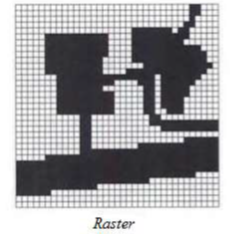
\includegraphics[width=0.45\textwidth]{raster.png} %% PARA COLOCAR O ARQUIVO DA IMAGEM NO SHARELATEX, CLIQUE NO ÍCONE QUE PARECE UMA FLECHINHA PARA CIMA (ATUALIZAR), CLIQUE EM UPLOAD E PROCURE A IMAGEM EM SEU COMPUTADOR.
\end{figure}

Nas estruturas vetoriais um número finito de segmentos em linha reta são definidos pelos seus pontos finais. A representação de um elemento ou objeto é uma tentativa de reproduzi-la o mais exatamente possível. Qualquer entidade ou elemento gráfico de um mapa é reduzido a três formas básicas: pontos, linhas ou polígonos. Caracteriza-se por ser uma representação adequada para uma ampla gama de dados espaciais sendo mais vantajoso que a matricial por armazenar pontos de interesse ao sistema (CÂMARA, 2005).

\begin{figure} [H] 
%% hbt SIGNIFICA QUE ELE PRIMEIRO VAI TENTAR COLOCAR A IMAGEM NESTE LUGAR (h de "here"). SENÃO DER, ELE TENTA COLOCAR MAIS PRA BAIXO (b de "bottom"). SENÃO ELE COLOCA MAIS PARA CIMA (t de "top").
\label{figura1} 
%% LABEL SERVE PARA VOCÊ REFERENCIAR A FIGURA NO MEIO DO TEXTO (VEJA LINHA 330: \ref{figura1}). ASSIM VOCÊ NÃO PERDE A REFERÊNCIA QUANDO MUDA A FIGURA DE LUGAR
\caption{Representação da estrutura vetorial}
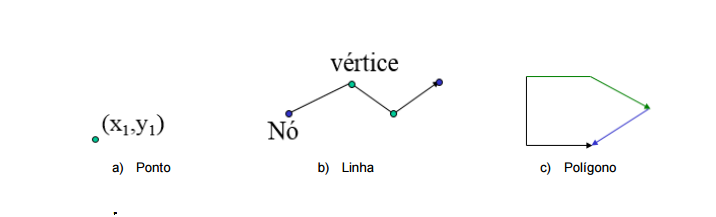
\includegraphics[width=0.95\textwidth]{vetorial.png} %% PARA COLOCAR O ARQUIVO DA IMAGEM NO SHARELATEX, CLIQUE NO ÍCONE QUE PARECE UMA FLECHINHA PARA CIMA (ATUALIZAR), CLIQUE EM UPLOAD E PROCURE A IMAGEM EM SEU COMPUTADOR.
\end{figure}

As diferenças entre os dados geográficos de estrutura vetorial e estrutura matricial são várias, como:

•	Precisão Geométrica: Os dados de estrutura vetorial possuem uma precisão geométrica maior que os dados de estrutura matricial;

•	Tamanho do arquivo: Os dados de estrutura vetorial necessitam de menor espaço em disco para serem armazenados;

•	Processamento: O processamento de dados matriciais é mais simples, os dados matriciais são indicados para o processamento de elementos da superfície contínua;

•	Exibição: Os dados de estrutura vetorial são mais rápidos para serem exibidos.

(PORQUE A ESCOLHA DO VETORIAL....)

Banco de Dados Geográficos
Os SIG precisam armazenar grandes quantidades de dados e torná-los disponíveis para operações de consultas e análise (LISBOA FILHO,). Com o aumento na procura por SIG, houve a necessidade de gerenciadores de dados geográficos que armazenam tanto a geometria como também os atributos dos objetos em um Sistemas Gerenciadores de Banco de Dados (SGBD) que são ferramentas fundamentais paro os SIG.

Os SIGs lidam com grandes quantidades de dados, e o armazenamento e manipulação desses dados tornam-se uma tarefa difícil devido à grande quantidade de informações. Desta forma, o uso de Sistemas de Gerenciamento de Banco de Dados é imprescindível na administração dessas informações.

O componente de armazenamento do SIG, denominado Banco de Dados Geográficos (BDG), estrutura e armazena os dados para possibilitar a realização das operações de análise e persistência de dados espaciais, capazes de descrever fenômenos geográficos cuja localização está relacionada a uma posição sobre a superfície terrestre (CÂMARA, 2005).
Existe um grande número de pesquisas na área de banco de dados voltadas a buscar novas formas de gerenciar dados georreferenciados. Atualmente, a estrutura mais utilizada na elaboração dos SIG é a que emprega um sistema dual. O SIG é composto de SGBD relacional, responsável pela gerência dos atributos acoplado a um componente de software responsável pelo gerenciamento dos atributos espaciais (LISBOA FILHO,).


% --- Seção dentro do capítulo
\section{Sistemas de Informação Geográfica na Web}

O SIG Web é um sistema que provê diferentes serviços de análise e visualização de dados espaciais, possibilitando um trabalho cooperativo entre pessoas, até mesmo em locais diferentes, que utilizem as mesmas informações consolidadas em um único ambiente. Caracterizando-se também por ser uma plataforma de gerenciamento que permite armazenar, analisar e manipular dados geográficos em ambiente web (Schimiguel, Baranauskas e Medeiros 2005).

Os SIGs são categorias de software que permitem a manipulação, gerenciamento e visualização de dados georreferenciados. Sistemas de Informação Geográfica na web são sistemas onde a informação geográfica pode estar dispersa em diferentes locais e sua manipulação via SIG ocorre através da Internet (SCHIMIGUEL, 2006).

O desenvolvimento de sistemas SIG web é complexo e deve considerar requisitos pouco encontrados em aplicações tradicionais: por exemplo, o grande volume de dados gerenciado (convencionais e georreferenciados), a diversidade de usuários no ambiente Web e processamento concorrente de requisições (BRESSAN, 2010).

A complexidade no desenvolvimento de um SIG web envolve Usabilidade, Acessibilidade e Interoperabilidade. Esses três termos devem caminhar juntos para resultar numa ferramenta capaz de atingir o uso por todas as pessoas (BRESSAN, 2010). Por se tratar de informação geográfica na web é importante saber a forma que a informação será trabalhada, para que mesmo o usuário leigo na área de geoprocessamento possa receber a informação de forma clara e objetiva.

Os SIG Web permitem que seja feita a divulgação de informações geográficas em larga escala, permitindo aos usuários da Internet o acesso a dados espaciais de forma facilitada, sem que haja a necessidade de serem especialistas no assunto.

Aplicações de Sistemas de Informação Geográfica na Web têm recebido grande destaque, por possibilitarem manipular e visualizar informações geográficas em diferentes locais, por diferentes perfis de usuários, através da Internet. Isso aumenta a complexidade da implementação de aplicações SIG, tanto com relação a aspectos funcionais quanto a aspectos de interface de usuário e interação humano-computador (IHC). Todo um avanço tecnológico, juntamente com recursos de programas voltados para o contexto de SIG e a disseminação da Internet no cotidiano, possibilitaram a interação com mapas na Internet. (SCHIMIGUEL, JULIANO et al, 2005).


% ---
\section{Ferramentas de Coleta de Dados}

Diversas ferramentas digitais têm sido amplamente utilizadas afim de aprimorar métodos que auxiliam na coleta de dados, tais como: QuickTapSurvey, aplicativo que tem a finalidade de tornar questionários e coletas de dados fáceis de manipular, permitindo que os usuários criem seus próprios questionários e coletem respostas sem depender de conexão à Internet. 
Outro exemplo é o DataGoal que trabalha com questionários digitais, enviando instantaneamente, dependendo da conexão com a Internet, as coletas de dados em campo para o servidor da base de dados das entrevistas, para realizar o acompanhamento em tempo real.

\begin{figure} [H] 
%% hbt SIGNIFICA QUE ELE PRIMEIRO VAI TENTAR COLOCAR A IMAGEM NESTE LUGAR (h de "here"). SENÃO DER, ELE TENTA COLOCAR MAIS PRA BAIXO (b de "bottom"). SENÃO ELE COLOCA MAIS PARA CIMA (t de "top").
\label{figura1} 
%% LABEL SERVE PARA VOCÊ REFERENCIAR A FIGURA NO MEIO DO TEXTO (VEJA LINHA 330: \ref{figura1}). ASSIM VOCÊ NÃO PERDE A REFERÊNCIA QUANDO MUDA A FIGURA DE LUGAR
\caption{\textit{Datagoal}}
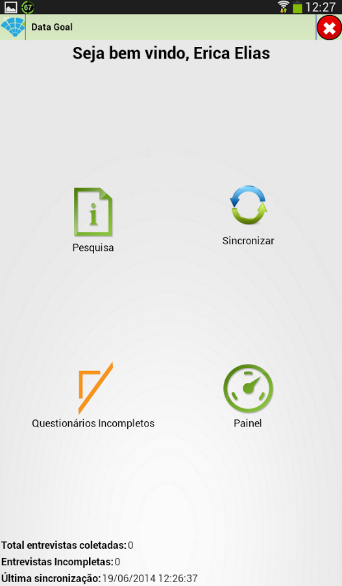
\includegraphics[width=0.45\textwidth]{datagoal.png} %% PARA COLOCAR O ARQUIVO DA IMAGEM NO SHARELATEX, CLIQUE NO ÍCONE QUE PARECE UMA FLECHINHA PARA CIMA (ATUALIZAR), CLIQUE EM UPLOAD E PROCURE A IMAGEM EM SEU COMPUTADOR.
\end{figure}

\begin{figure}[H]

\minipage{0.26\textwidth}
  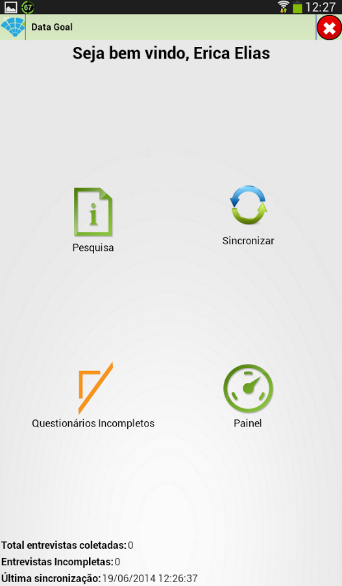
\includegraphics[width=0.105\linewidth]{datagoal.png}
  \caption{\scriptsize Adolescentes.}\label{fig:awesome_image1}
\endminipage\hfill
\minipage{0.26\textwidth}%
  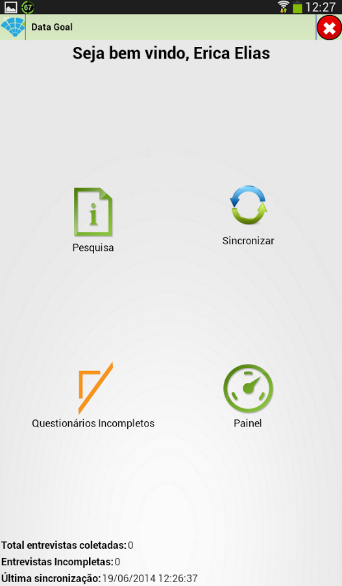
\includegraphics[width=0.45\linewidth]{datagoal.png}
  \caption{\scriptsize Idosos.}\label{fig:awesome_image3}
\endminipage

\end{figure}

\section{Aplicações SIG na Web}

Tecnologias SIG web têm sido amplamente utilizadas, com propósito de permitir que as informações geográficas sejam divulgadas em grande alcance através da Internet de forma rápida e fácil. Exemplo de algumas aplicações que utilizam o dinamismo da Internet com o SIG Web para divulgar dados e informações importantes:


\begin{figure} [H] 
%% hbt SIGNIFICA QUE ELE PRIMEIRO VAI TENTAR COLOCAR A IMAGEM NESTE LUGAR (h de "here"). SENÃO DER, ELE TENTA COLOCAR MAIS PRA BAIXO (b de "bottom"). SENÃO ELE COLOCA MAIS PARA CIMA (t de "top").
\label{figura1} 
%% LABEL SERVE PARA VOCÊ REFERENCIAR A FIGURA NO MEIO DO TEXTO (VEJA LINHA 330: \ref{figura1}). ASSIM VOCÊ NÃO PERDE A REFERÊNCIA QUANDO MUDA A FIGURA DE LUGAR
\caption{\textit{Wikicrimes}}
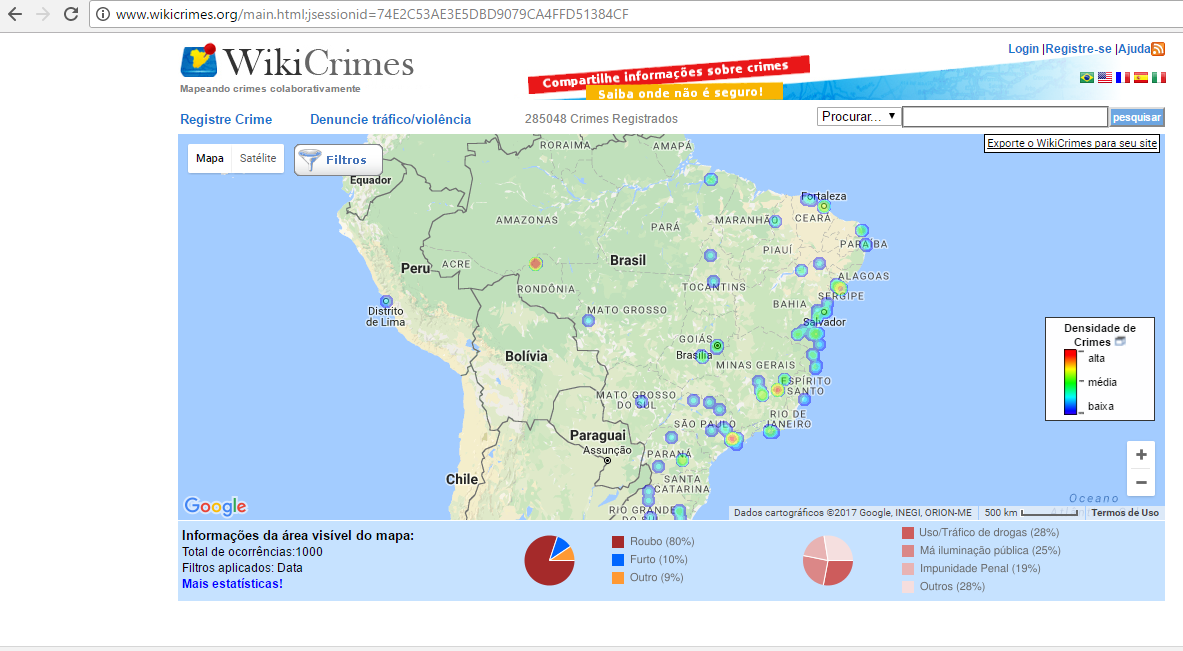
\includegraphics[width=0.95\textwidth]{wikicrimes.png} %% PARA COLOCAR O ARQUIVO DA IMAGEM NO SHARELATEX, CLIQUE NO ÍCONE QUE PARECE UMA FLECHINHA PARA CIMA (ATUALIZAR), CLIQUE EM UPLOAD E PROCURE A IMAGEM EM SEU COMPUTADOR.
\end{figure}

\textit{\textbf{Wikicrimes}} trabalha com crimes mapeados, onde permite o mapeamento de crimes através de cadastros e identificações de zonas perigosas mostrando estatísticas, contribuindo como um infortivo, previndo que as pessoas circulem por zonas perigosas.

\begin{figure} [H] 
%% hbt SIGNIFICA QUE ELE PRIMEIRO VAI TENTAR COLOCAR A IMAGEM NESTE LUGAR (h de "here"). SENÃO DER, ELE TENTA COLOCAR MAIS PRA BAIXO (b de "bottom"). SENÃO ELE COLOCA MAIS PARA CIMA (t de "top").
\label{figura1} 
%% LABEL SERVE PARA VOCÊ REFERENCIAR A FIGURA NO MEIO DO TEXTO (VEJA LINHA 330: \ref{figura1}). ASSIM VOCÊ NÃO PERDE A REFERÊNCIA QUANDO MUDA A FIGURA DE LUGAR
\caption{\textit{Rumsey}}
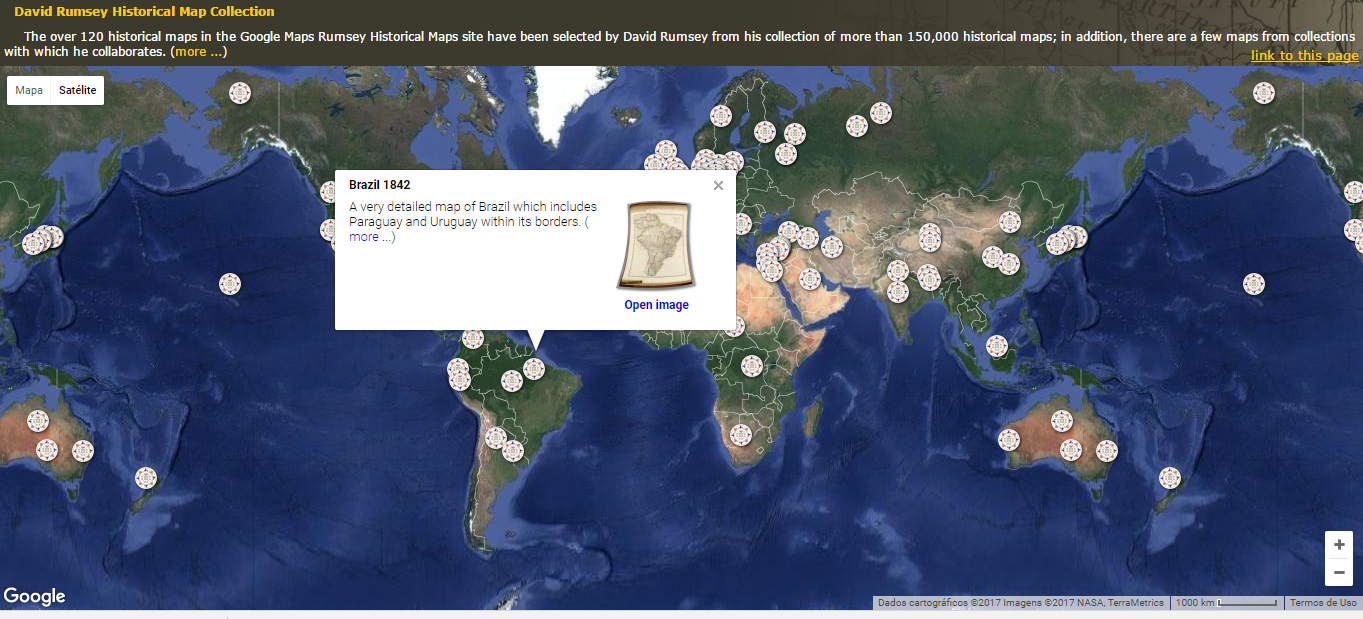
\includegraphics[width=0.95\textwidth]{rumsey.png} %% PARA COLOCAR O ARQUIVO DA IMAGEM NO SHARELATEX, CLIQUE NO ÍCONE QUE PARECE UMA FLECHINHA PARA CIMA (ATUALIZAR), CLIQUE EM UPLOAD E PROCURE A IMAGEM EM SEU COMPUTADOR.
\end{figure}

\textit{\textbf{Rumsey}} Disponibiliza mapas históricos, onde fornece uma coleção de mais de 150.000 mapas históricos. 

\begin{figure} [H] 
%% hbt SIGNIFICA QUE ELE PRIMEIRO VAI TENTAR COLOCAR A IMAGEM NESTE LUGAR (h de "here"). SENÃO DER, ELE TENTA COLOCAR MAIS PRA BAIXO (b de "bottom"). SENÃO ELE COLOCA MAIS PARA CIMA (t de "top").
\label{figura1} 
%% LABEL SERVE PARA VOCÊ REFERENCIAR A FIGURA NO MEIO DO TEXTO (VEJA LINHA 330: \ref{figura1}). ASSIM VOCÊ NÃO PERDE A REFERÊNCIA QUANDO MUDA A FIGURA DE LUGAR
\caption{\textit{Healtmap}}
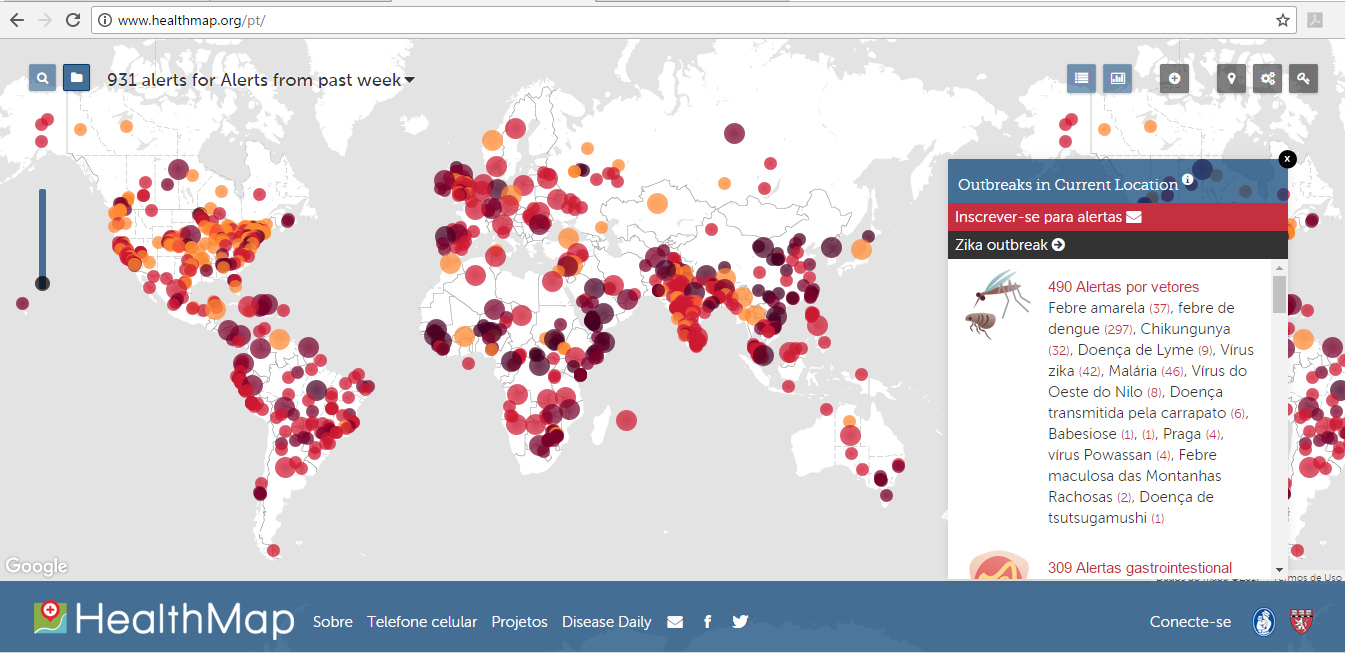
\includegraphics[width=0.95\textwidth]{healt.png} %% PARA COLOCAR O ARQUIVO DA IMAGEM NO SHARELATEX, CLIQUE NO ÍCONE QUE PARECE UMA FLECHINHA PARA CIMA (ATUALIZAR), CLIQUE EM UPLOAD E PROCURE A IMAGEM EM SEU COMPUTADOR.
\end{figure}

\textit{\textbf{Healtmap}} Fornece o estado atual de doenças e seus efeitos em seres humanos e animais em todo o mundo. As informações são atualizadas a todo tempo pela Organização Mundial de Saúde.

\chapter{Trabalhos Relacionados}
Existem ferramentas digitais com o propósito de aprimorar os métodos que auxiliam na coleta de dados. A ferramenta \textit{Data Goal}, trabalha com questionários digitais, enviando de imediato, se existir conexão com à Internet, os dados coletados em campo para um servidor da base de dados das entrevistas para acompanhamento em tempo real. O diferencial positivo em relação ao \textit{Data Goal} é a não depência à conexão com a \textit{Internet}.

O \textit{QuickTapSurvey}, facilita a criação de questionários e coletas de dados de forma interativa permitindo que os usuários criem seus próprios questionários e coletas de dados de forma interativa, permitindo assim, os usuários criarem seus próprios questionários e coletem respostas sem depender de conexão à Internet.

O Nokia Data Gathering é um sistema que provê a criação de questionários móveis que, colocados em um servidor na Internet, podem ser acessados pelos dispositivos móveis com acesso à rede. Os dados são coletados e armazenados nos dispostivos e podem ser transmitidos para um servidor. 

Um projeto similar que devemos citar é o Maritaca que consiste numa arquitetura de construção de aplicações para coleta de dados usando dispositivos móveis; os usuários têm a liberdade de construir seus questionários compostos por diversas perguntas. Nos dispositivos móveis, o aplicativo permite a coleta de dados utilizando interfaces amigáveis, onde os dados são armazenados nos smartphones até serem transferidos para o servidor, sem que haja conexão à internet para a coleta. Entretanto a criação fica restrita ao navegador web.

Um ponto diferencial da arquitetura proposta é a criação dos questionários customizados e a coleta é feita pela aplicação móvel, e poderá ser armazenada informações de localização geográfica; e a \textit{interfece web} será responsável por prover meio de exibição dos dados coletados e oferece mecanismos de consultas geográficas utilizando a ferramenta SIG acoplada.

Conforme observado, existem trabalhos semelhantes ao projeto que está sendo proposto. Entretanto, não tratam de todos os pontos apresentados nesta arquitetura, que tem como intuito permitir ao usuário maior capacidade de manipulação de suas informações através de diversas funcionalidades.



\chapter{Desenvolvimento da Aplicação}
A proposta desse trabalho consiste na criação de uma \textit{Interface web} para exibição e manipulação das informações geográficas, que compõe um dos quatro módulos de uma arquitetura para coleta de questionários customizados georreferenciados. Essa arquitetura é caracterizada por permitir o armazenamento da localização geográfica dos questionários coletados, a capacidade de customização das sequências de perguntas e a manipulação dos dados georreferenciados.

Os módulos da arquitetura foram assim determinados: 

•	Modelagem de um banco de dados geográficos; 

•	Desenvolvimento de uma ferramenta SIG para suporte;

•	Desenvolvimento de uma \textit{interface web} para visualização;

•	Desenvolvimento de uma aplicação móvel de coleta.


A visualização dos questionários será feita pelo SIG Web, com o propósito de exibir os dados que forem obtidos pelo aplicativo \textit{Android} nas pesquisas de campo. Essa \textit{Interface} será responsável por prover meios para visualizar a distribuição espacial destes dados, podendo realizar consultas geográficas e filtros de perguntas.

Inicialmente, para o desenvolvimento da \textit{Interface} de apresentação, foi necessária a modelagem de uma ferramenta SIG e também a modelagem e implementação do banco de dados geográficos que deu suporte à execução do projeto. 

Foram realizados testes sobre o banco de dados já implementado que envolveram a criação de questionários fictícios e realizados consultas geográficas na ferramenta SIG desenvolvida. Dessa maneira a aplicação foi desenvolvida utilizando as seguintes tecnologias:

•	Modelagem do Banco de Dados Geográfico – Foi utilizado o banco de dados PostgreSQL com a extensão espacial PostGIS. A integração do Banco de Dados (BD) com a extensão espacial acontece de forma transparente para o usuário, mas complexa internamente. O PostGIS fornece a ligação do BD com os tipos de dados espaciais, e permite o uso de objetos do SIG;

•	Ferramenta SIG – A ferramenta SIG servirá para manipular os dados geográficos que forem armazenados no banco de dados. A modelagem de teste para a ferramenta foi feita em ambiente web utilizando a linguagem de programação PHP, que é uma linguagem livre responsável pela conexão do banco de dados PostgreSQL com A API Google Maps, sendo o conteúdo e resultado dessa conexão visualizado diretamente al algum navegador. A versão utilizada do PHP foi 5.5.12 compilada com o servidor web Apache 2.4.9.

o	A API Google Maps interage com o PHP obtendo respostas da conexão usando retorno de dados. Foi a ferramenta utilizada para visualizar mapas e acessar recursos avançados de mapeamento, como exibição de polígonos, pontos, dentre outros.

o	Para aprofundar nos conhecimentos dos recursos dos SIGs, e colocar em prática na API do Google Maps, foram utilizadas algumas ferramentas de software SIG: o gvSIG e QGIS.


\section{Diagrama Entidade Relacionamento}


\begin{figure} [H] 
%% hbt SIGNIFICA QUE ELE PRIMEIRO VAI TENTAR COLOCAR A IMAGEM NESTE LUGAR (h de "here"). SENÃO DER, ELE TENTA COLOCAR MAIS PRA BAIXO (b de "bottom"). SENÃO ELE COLOCA MAIS PARA CIMA (t de "top").
\label{figura1} 
%% LABEL SERVE PARA VOCÊ REFERENCIAR A FIGURA NO MEIO DO TEXTO (VEJA LINHA 330: \ref{figura1}). ASSIM VOCÊ NÃO PERDE A REFERÊNCIA QUANDO MUDA A FIGURA DE LUGAR
\caption{Diagrama Entidade Relacionamento}
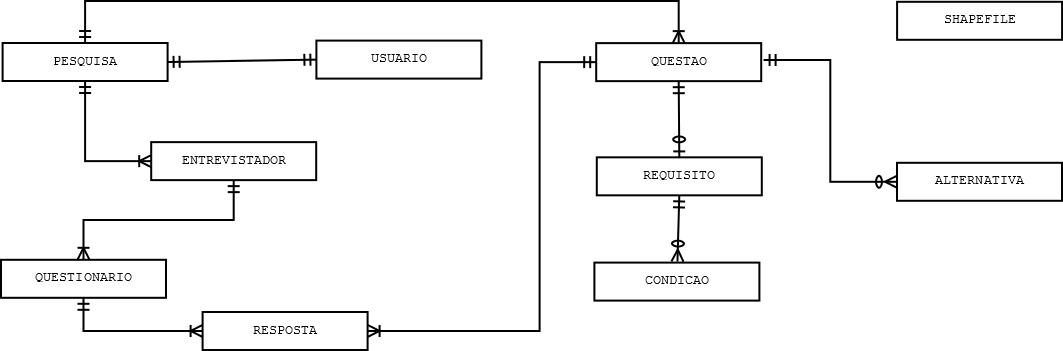
\includegraphics[width=0.95\textwidth]{diagrama.png} %% PARA COLOCAR O ARQUIVO DA IMAGEM NO SHARELATEX, CLIQUE NO ÍCONE QUE PARECE UMA FLECHINHA PARA CIMA (ATUALIZAR), CLIQUE EM UPLOAD E PROCURE A IMAGEM EM SEU COMPUTADOR.
\end{figure}

Adiante, será explicada a modelagem e tabelas utilizadas pelo sistema de questionário:

\begin{table}[H!]
\caption{My table caption 1.}
\label{my-label}


\begin{center}
\begin{tabular}{llp{13cm}} 
    \hline
    Tabela & Descrição \\
    \hline
    \\
    Usuário  & \parbox{13cm}{Nesta tabela é feito um cadastro simples de usuários, com dados como nome, idade, e-mail, senha etc. O e-mail e senha informados servirão para autenticação dos usuários para acesso de seus questionários posteriormente. A tabela deriva dois tipos de usuários existentes: pesquisador ou entrevistador.} 
    \\
    \\
    \hline
    \\
    Pesquisa  & \parbox{13cm}{Atividade designada ao pesquisador, e não deve ser confundida com questionário. Esta tabela conterá as descrições da pesquisa a ser desenvolvida pelo pesquisador, exemplo, Pesquisa sobre a Dengue. A partir da pesquisa criada poderão ser criados diferentes questionários.} 
    \\
    \\
    \hline
    \\
    Entrevistador & \parbox{13cm}{Usuário que tem a função de aplicar os questionários associado às pesquisas criadas. Só tem acesso ao questionário que aplicou.}
    \\
    \\
    \hline
    \\
    Questionário  & \parbox{13cm}{ É a aplicação da pesquisa que foi desenvolvida pelo entrevistador. Ao criar um questionário, será definido o entrevistador que aplicará os questionários, a data e a localização geográfica por meio das coordenadas espaciais do local onde está sendo aplicado o questionário. Para acessar os questionários, o pesquisador só poderá ter acesso aos questionários referentes à sua pesquisa, aplicados por diferentes entrevistadores.}
    \\
    \\
    \hline
    \\
    Questão & \parbox{13cm}{Para desenvolver as questões, é importante que o pesquisador esteja ciente na lógica do desenvolvimento das questões, ou seja, desenvolver perguntas que levem a um objetivo específico. A organização das perguntas das questões é de suma importância pois no nosso sistema, a sequência de perguntas pode ser influenciada por respostas anteriores. Considerando os requisitos e condições de cada pergunta. Existe um suporte à criação de perguntas fechadas e abertas.}
    \\
    \\
    \hline
    \\
    Alternativa & \parbox{13cm}{Estão relacionadas as perguntas das questões fechadas.}
    \\
    \\
    \hline
    \\
    Requisito & \parbox{13cm}{Nesta tabela circula toda a lógica de transição entre as questões durante a aplicação do questionário. Está inserida na tabela a origem e o destina das questões. A origem é a questão que tem condições que, quando satisfeitas, direcionam a aplicação à próxima pergunta, que é o destino. Estes requisitos devem ser cuidadosamente implementados, para que não haja falhas de condições.}
    \\
    \\
    \hline
    \\
    Condição & \parbox{13cm}{É uma restrição que deve ser satisfeita em uma resposta a uma questão, para que haja transação para a próxima questão. Cada questão pode ter vários tipos de requisitos, ou seja, mais de um requisito pode ser elaborado, podendo existir diferentes tipos de condições para cada requisito. Além disso, pode existir a possibilidade de uma questão possuir mais de uma origem, dessa forma a construção deve ser bastante rigorosa.}
    \\
    \\
    \hline
    \\
    Resposta & \parbox{13cm}{São armazenada nessa tabela as respostas de cada pergunta referente ao questionário aplicado pelo entrevistador. Caso seja uma questão aberta, será mostrado a resposta descrita pelo entrevistado. Se for uma questão fechada, será armazenada a alternativa escolhida. Serão armazenadas e disponíveis para exibição apenas as perguntas respondidas.}
    \\
    \\
    \hline
    \\
    Shapefile & \parbox{13cm}{Esta tabela está à disposição para receber os shapefiles, que é o formato de armazenagem de dados vetoriais para armazenar a posição, formato e atributos de feições geográficas. Ele irá receber shapefiles de múltiplos polígonos, que futuramente estarão disponíveis para fazer upload pelos entrevistadores e pesquisadores.}
    \\
    \\
    \hline
    \\
 \end{tabular}
 \end{center}
 \end{table}


\section{Arquitetura de Coleta de Questionários}

O ponto diferencial da arquitetura para a coleta de questionários, é poder dar a liberdade para a customização de seus questionários, ou seja, definindo diferentes fluxos de sequência para as perguntas e suas distribuições espaciais. Sendo uma opção importante na aplicação de pesquisas diante diferentes perfis de usuários, tornando assim o processo flexível e levando ao foco das perguntas de interesse.


Como já mencionado a arquitetura de coleta de questionários customizados é composta por quatro módulos.

\begin{figure} [H] 
%% hbt SIGNIFICA QUE ELE PRIMEIRO VAI TENTAR COLOCAR A IMAGEM NESTE LUGAR (h de "here"). SENÃO DER, ELE TENTA COLOCAR MAIS PRA BAIXO (b de "bottom"). SENÃO ELE COLOCA MAIS PARA CIMA (t de "top").
\label{figura1} 
%% LABEL SERVE PARA VOCÊ REFERENCIAR A FIGURA NO MEIO DO TEXTO (VEJA LINHA 330: \ref{figura1}). ASSIM VOCÊ NÃO PERDE A REFERÊNCIA QUANDO MUDA A FIGURA DE LUGAR
\caption{Estrutura da Arquiteura}
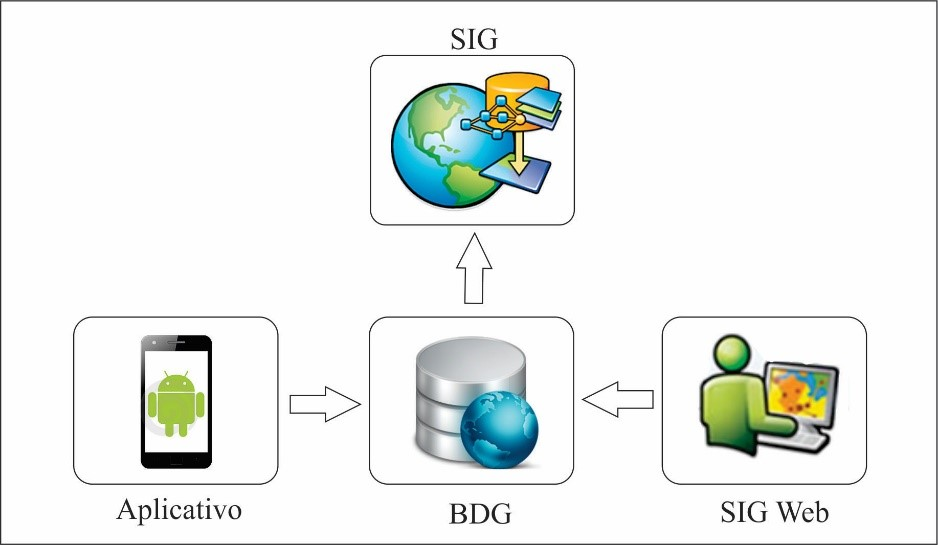
\includegraphics[width=0.95\textwidth]{arquituraproposta.jpg} %% PARA COLOCAR O ARQUIVO DA IMAGEM NO SHARELATEX, CLIQUE NO ÍCONE QUE PARECE UMA FLECHINHA PARA CIMA (ATUALIZAR), CLIQUE EM UPLOAD E PROCURE A IMAGEM EM SEU COMPUTADOR.
\end{figure}

É representado na figura acima a estrutura da arquitetura. Composta por um \textbf{Banco de Dados Geográfico} que servirá como base para a implementação do projeto, e serão armazenados dados coletados dos questionários incluindo as localizações geográficas.

\textbf{A ferramenta SIG} servirá como o suporte para a arquitetura por meio de suas ferramentas para coletar, armazenar, manipular, e analisar as informações. A base de dados permitirá a interpretação segundo diferentes visões. 

A visualização dos questionários será feita pelo \textbf{SIG Web}, com o propósito de exibir os dados que forem obtidos pelo aplicativo Android nas pesquisas de campo. Essa \textit{Interface} é responsável por prover meios para visualizar a distribuição espacial destes dados, podendo realizar consultas geográficas e filtros de perguntas.

A criação dos questionários customizados será realizado por meio de um \textbf{Aplicativo} desenvolvido na plataforma \textit{Android}. A aquisição dos dados é realizada através da tecnologia do GPS, pois possibilita a realização de levantamentos de campo com alto grau de precisão sem dependência de conexão à \textit{Internet} .


O desenvolvimento desse trabalho que compõe um módulo da arquitetura de coleta de questionários customizados têm o propósito de criar uma \textit{Interface Web} que visualize os dados desses questionários, como uma forma de apresentação dos resultados obtidos através da coleta. Serão permitidas por meio dessa Interface proposta a realização das consultas geográficas, e a manipulação da ferramenta SIG acoplada.

As atividades de cadastro de usuários, criação de questionários será realizado pelo Aplicativo, em desenvolvimento, e não cabe à Interface web a execução dessas tarefas. Ficando responsável apenas para a exibição, pois, o interesse maior é mostrar aos diferentes perfis usuários que a informação geográfica pode ser manipulada e visualizada em diferentes locais por meio da web.



% ---
% Conclusão
% ---
\chapter{Conclusão}

A procura por informação geoespacial cresceu bastante pela popularização dos dispositivos móveis, e com isso a evolução dos Sistemas de Informação Geográficos se tornaram mais presentes no cotidiano das pessoas.

Considerando que o propósito inicial deste trabalho consiste na criação de uma interface web de visualização dos dados georreferenciados que serão coletados por meio de uma ferramenta móvel de coleta, nota-se que foi possível obter os resultados desejados acerca da proposta.

Uma proposta de estilização de uma página web afim de levar os usuários deste projeto a uma maior comodidade para visualizar as pesquisas e questionários realizados.
Vale ressaltar que uma parte da página web já tinha sido implementada anteriormente por outro membro do projeto, pois necessitava da criação para a implantação das tecnologias SIGs aplicadas por ela. Esse trabalho consistiu na continuação do mesmo, trazendo uma fluidez à página e otimizando-a.

A Grandiosidade deste projeto e o alcance que ele pode chegar é muito positivo, pois o objetivo é dar a liberdade de que seus usuários criem as pesquisas de acordo com o interesse próprio, em suas atividades de campo, observando diretamente os fenômenos geográficos sob diferentes pontos de vista.

Os testes realizados das consultas geográficas com questionários fictícios mostraram resultados satisfatório no que se diz respeito a lógica de customização proposta pelo projeto. Mostraram eficiência e agilidades com as ferramentas espaciais, como também ao banco de dados geográficos acoplado.

Como trabalhos futuros, está planejado o desenvolvimento da aplicação do sistema Android para os dispositivos móveis, que dará suporte à coleta de questionários customizados, permitindo aos usuários a criação dos questionários e a coleta dos dados.
(INCOMPLETO).


\chapter{Publicações}
Caso o aluno possua publicações de artigos científicos, estes deverão ser listados neste capítulo.

% ----------------------------------------------------------
% ELEMENTOS PÓS-TEXTUAIS
% ----------------------------------------------------------
\postextual


% ----------------------------------------------------------
% Referências bibliográficas
% ----------------------------------------------------------
\bibliography{references} %% REFERENCIA AO ARQUIVO abntex2-modelo-references.bib

% ----------------------------------------------------------
% Glossário
% ----------------------------------------------------------
%
% Consulte o manual da classe abntex2 para orientações sobre o glossário.
%
%\glossary

% ----------------------------------------------------------
% Apêndices
% ----------------------------------------------------------

% ---
% Inicia os apêndices
% ---
\begin{apendicesenv}

% Imprime uma página indicando o início dos apêndices
\partapendices

% ----------------------------------------------------------
\chapter{Apêndice}
% ----------------------------------------------------------


\end{apendicesenv}
% ---



\end{document}
